\section{Experiments}\label{sec:experiments}
We demonstrate that \NAME{} can improve performance in low-SNR videos across medical and ecological applications (\cref{sec:results}). We evaluate our processed images on downstream tasks for detection, tracking, counting, and classification. 

\subsection{Datasets} \label{sec:datasets}

\textbf{Caltech Fish Counting 2022}  (CFC22) \cite{cfc2022eccv} is designed for detection, tracking, and counting fish in low-signal-to-noise sonar video. This dataset contains 1,567 sonar videos from seven different cameras on three rivers in Alaska and Washington. The videos are grayscale, their resolutions range from 288x624 to 1,086x2,125, their frame rates range from 6.7 to 13.3 fps, and each video is on average 336 frames (38s) in duration \cite{cfc2022eccv}. In total, there are 527,215 frames with 8,254 unique fish, totaling 516k bounding boxes and 16.7 hours of video \cite{cfc2022eccv}.  The dataset includes significant domain shifts (\eg, background topology, occlusion, fish densities, fish sizes, camera noise), requiring models to generalize effectively across conditions. 

\noindent{}\textbf{Breast Lesion Ultrasound Video Dataset} \cite{CVANet} (BUV) is designed for classifying (benign or malignant) and localizing breast lesions. The dataset contains 188 videos, of which 113 are malignant and 75 are benign. These videos collectively have 25,272 images, each with 1 detection; the number of ultrasound images in each video range from 28 to 413. Each video has a complete scan of the abnormal tissue. The dataset has a random train--test split of 150--38 videos respectively\cite{CVANet}.

\noindent{}\textbf{The Point-of-care Ultrasound dataset (POCUS)} \cite{born2021accelerating, born2021l2} contains convex and linear probe lung ultrasound images and videos for classifying COVID-19 and pneumonia. It includes 247 videos and 59 images; we use only the videos. Of these, 70 show COVID cases, 45 \textit{possible} COVID, 51 bacterial pneumonia, 6 viral pneumonia, and 75 healthy lungs. Videos are sampled at 10Hz, and frames are grouped by video as in Born et al. \cite{born2021accelerating, born2021l2}. In total, we extract 9,184 frames with an average size of 499×463 pixels.

\noindent{}\textbf{Fluorescence microscopy dataset} \cite{ulman2017objective} (Fluo) is a dataset of fluorescence-microscopy recordings of live cells in \cite{ulman2017objective}. We use the same videos as UDVD \cite{Sheth_2021_ICCV}: Fluo-32DL-MSC (CTC-MSC), of mesenchymal stem cells, and Fluo-N2DH-GOWT1 (CTC-N2DH), of GOWT1 cells. This dataset also contains no ground-truth clean data. There are a total of 560 frames and four videos. 

\subsection{Training Procedure -- Denoiser}
We train \NAME{} using the reconstruction objective in \cref{eqn:recon_loss}. During training, we rescale CFC22 and POCUS images to 1024x512 and BUV and Fluo images to 1024x1024. For POCUS, we use a sample rate of 10Hz, as that is what the downstream process uses. For all other datasets, we use all frames. Because SAVeD is self-supervised, when training the \textit{denoiser} for each dataset, we train over all data. We train for 20 epochs for CFC22, 120 epochs for POCUS, 40 epochs for BUV, and 1000 epochs for Fluo; we found these numbers of epochs sufficient for training to converge. These took 20 hours, 0.5 hours, 2 hours, and 2 hours, respectively, on 2 RTX 4090 GPUs; this is less time than other network-based denoising methods as seen in \cref{tab:denoiser_time}. Additional details, including hyperparameter configurations, are in the Supplemental Materials \cref{sec:our_denoiser_hyperparams_and_details}.

After training \NAME{}, we generate denoised frames for all splits. In the case of CFC22, we combine the denoised image as two channels and the background-subtracted frame, $(I_v)_t - \bar{I_v}$, as the last channel. For POCUS, BUV, and Fluo, we combine the denoised image as two channels and the median-filtered image as the last channel. 
\begin{figure*}[t]
    \centering
    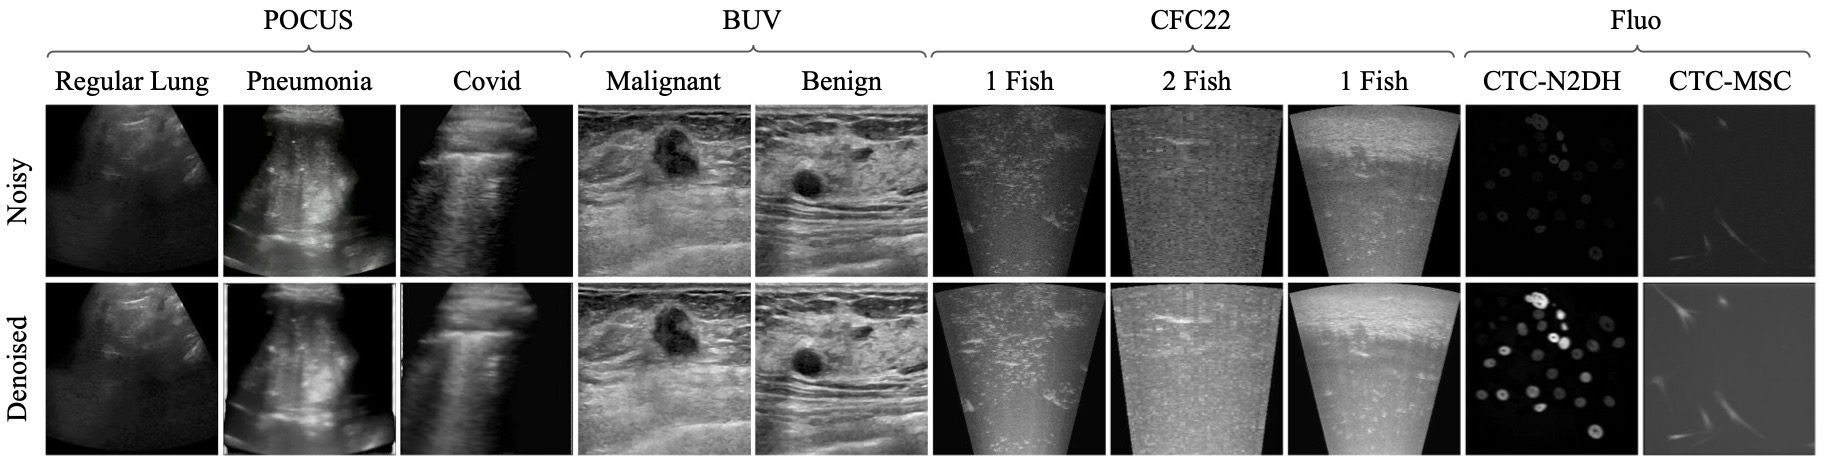
\includegraphics[width=\linewidth]{figs/qualitative_pairs4.jpg}
    \caption{\textbf{Qualitative raw-denoised pairs of \NAME{}}. Qualitative results for \NAME{} trained on POCUS (lung health categorization), BUV (breast lesion detection), CFC22 (fish detection, tracking, and counting), and Fluo (cell denoising).}
    \label{fig:qualitative_pairs}
\end{figure*}

\subsection{Evaluation procedure -- Downstream Tasks}
Given that none of our videos have clean (noise-free) versions, we use the downstream performance tasks' metrics as proxies for our denoised performance. We use $FBD$ from \cref{sec:denoising_metric} when detection annotations are available.

\textbf{Denoising for Detection, Tracking, and Counting.} For CFC22, which has detection, tracking, and counting as downstream tasks, we follow a simplified version of the detection pipeline from \citet{cfc2022eccv} -- we train a YOLOv5 model for 5 epochs with the longest side of an image set to 896 and no augmentations. We remove duplicate predictions using non-maximal suppression. We use mAP$_{50}$ \cite{map50} to evaluate detection performance frame-by-frame. We use a pretrained-frozen ByteTrack tracker and calculate MOTA \cite{clear}, HOTA \cite{HOTA}, and IDF1 \cite{IDF1} scores for evaluation. More details and hyperparameter settings are in the Supplemental Materials Sec. \ref{sec:cfc_detector_hyperparams} and \ref{sec:cfc_tracker_hyperparams}.  
For counting, we use trajectories from the tracks to create nMAE scores, defined in \citet{cfc2022eccv}, for each domain. The tracking and counting pipelines are training-free.

For BUV, we follow the training procedure of \citet{CVANet}; we also follow their final fine-tuning step and evaluation to generate an AP$_{50}$ metric. Note that we know that breast lesions are darker (rather than brighter) spots in ultrasounds. As a result, we invert our reconstruction error to take the minimum difference rather than the maximum: 
\begin{equation}
\text{inv}S_{t,T} = \min(0, I_{t+T} - I_t) + I_t + \min(0, I_{t-T} - I_t)
\end{equation}
\noindent{}\textbf{Denoising for Classification.} 
For POCUS, we perform 5-fold cross-validation following \citet{born2021accelerating, born2021l2}, ensuring all frames from a video remain in the same fold. We adopt their fine-tuning strategy and hyperparameters. For evaluation, we compute per-class precision, recall, and F1, then average across folds to obtain overall metrics.

 % \textit{Video classification.} Born et. al. also explored the temporal dimension of the videos with 3D convolutions. We follow their procedure on all folds.




